\documentclass[amssymb, amsmath]{beamer}
\usepackage[utf8]{inputenc}

\usepackage{utopia} %font utopia imported
\usepackage{color}
\usepackage{hyperref}
\usepackage{braket}
%\usepackage{dsfont}

\usetheme{AnnArbor}
\usecolortheme{wolverine}

\definecolor{suoh}{RGB}{126, 38, 57}
\definecolor{midori}{RGB}{42, 96, 59}
\definecolor{ruri}{RGB}{31, 71, 136}
\definecolor{iris}{RGB}{118, 53, 104}

\newcommand{\zhliu}[1]{\textcolor{iris}{#1}}
\newenvironment{zhenghao}{\color{iris}}{\color{black}}


\title[Group talk] %optional
{OAM Rotation detecting}

\subtitle{}

\author[Zhenghao Liu] % (optional)
{Zhenghao Liu\inst{1} \inst{2}}

\institute[] % (appears in parenthesis at bottom left block.)
{
  \inst{1}%
  Key Laboratory of Quantum Informaion, CAS
  \and
  \inst{2}%
  University of Science and Technology of China
}

\date[\today] % (optional)
{Group Meeting $@$ 04, Jun, 18}

\logo{}

%End of title page configuration block
%------------------------------------------------------------



%------------------------------------------------------------
%The next block of commands puts the table of contents at the 
%beginning of each section and highlights the current section:

\AtBeginSection[]
{
  \begin{frame}
    \frametitle{Table of Contents}
    \tableofcontents[currentsection]
  \end{frame}
}
%------------------------------------------------------------


\begin{document}

%The next statement creates the title page.
\frame{\titlepage}


%---------------------------------------------------------
%This block of code is for the table of contents after
%the title page
\begin{frame}
\frametitle{Table of Contents}
\tableofcontents
\end{frame}
%---------------------------------------------------------


\section{Operations on OAM state}

\begin{frame}
\frametitle{Operations on OAM states}

\begin{itemize}
    \item Spatial propagating: $\ket{m}\to\ e^{\frac{2\pi d}{\lambda}}\ket{m}$
    \item Mirror image: $\ket{m}\to\ket{-m}$
    \item Rotating by $\theta$: $\ket{m}\to e^{im\theta}\ket{m}$
    \item Rotated by \textcolor{suoh}{Dove prism} (@angle $\theta$): $\ket{m}\to e^{i2m\theta}\ket{-m}$
\end{itemize}
\end{frame}

\begin{frame}{Operations on OAM states: passing through cavity}
    
    State prepared is $\ket{\phi(t)}=e^{i m\Omega t}\ket{m}+e^{-i m\Omega t}\ket{-m}$. Mirror's amplitude transmittance set to be $T$, and cavity have free spatial range(FSR) $\nu_{FSR}$: 
\begin{columns}
\column{0.72\textwidth}
\begin{align}
\label{eq:psiorig}
    \ket{\psi(t)} &= \sum_{k=0}^{+\infty} (1-T)^k T \Ket{\phi\left(t-\frac{k}{\nu_{FSR}}\right)} \nonumber \\
    =& \frac{T e^{i m \Omega t} \ket{m}}{1-(1-T)e^{-i m \Omega / \nu}} \nonumber \\ 
    &+ \frac{T e^{-i m \Omega t} \ket{-m}}{1-(1-T)e^{i m \Omega / \nu}} 
\end{align}
Fig: a cavity blending up source emission of different times. Output is guaranteed to be constructive interference, but of different OAM states.

\column{0.28\textwidth}
\begin{figure}
    \centering
    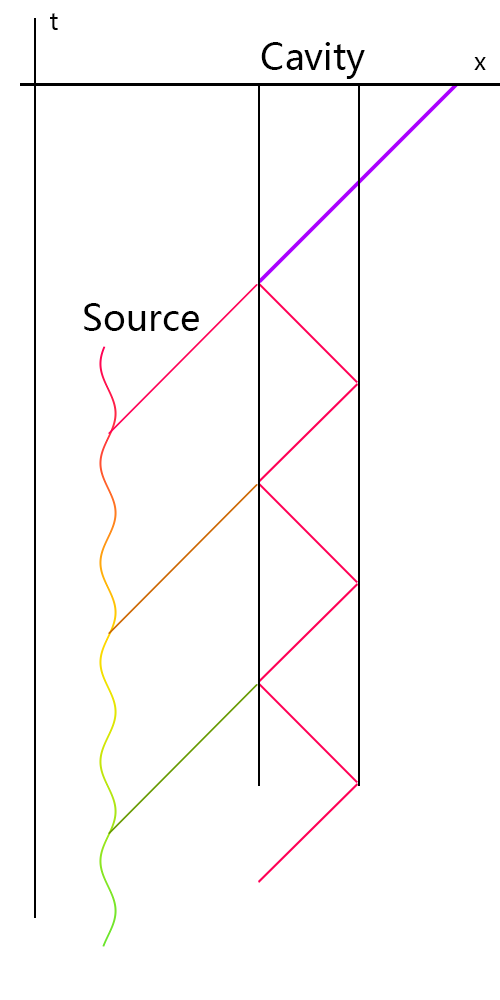
\includegraphics[width=0.80\columnwidth]{fig/cav_blend.png}
\end{figure}
\end{columns}
    
\end{frame}

\begin{frame}
\frametitle{Operations on OAM states: passing through cavity}

    In practice $T\ll1$ and $\Omega\ll\nu_{FSR}$, (\ref{eq:psiorig}) yields:
\begin{align}
    \ket{\psi(t)} &= \left(1-i\frac{m \Omega}{\nu_{FSR}T}\right)e^{i m \Omega t}\ket{m}
    +\left(1+i\frac{m \Omega}{\nu_{FSR}T}\right)e^{-i m \Omega t}\ket{-m} \\
    &\approx \Ket{\phi\left(t-\frac{1}{\nu_{FSR} T}\right)}=\ket{\phi(t^\prime)}
    \end{align}
\textcolor{midori}{Result: cavity effectively delays propagation of OAM state by $\frac{1}{\nu_{FSR} T}$}.

\end{frame}

\section{OAM mimicking Faraday rotation}

\begin{frame}
\frametitle{Article}

\begin{figure}
    \centering
    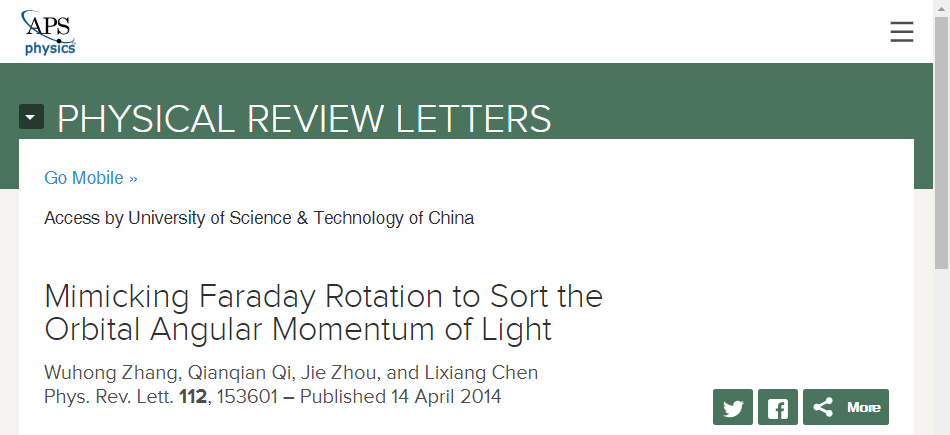
\includegraphics[width=0.80\columnwidth]{fig/title.png}
    \caption{PRL 112 153601, article to be discussed.}
\end{figure}

\end{frame}

\begin{frame}
\frametitle{Experimental Scheme}
\begin{figure}
    \centering
    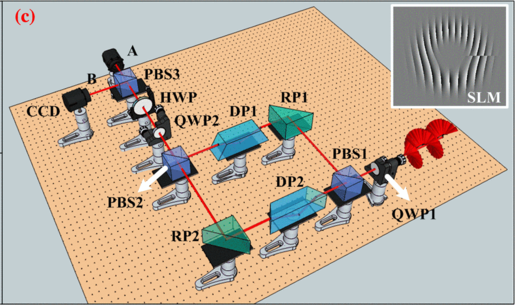
\includegraphics[width=0.80\textwidth]{fig/scheme_large.png}
    \caption{Experimental Scheme of Chen et. al, published on PRL(2014)}
    \label{fig:scheme_PRL}
\end{figure}

\end{frame}
%---------------------------------------------------------

\begin{frame}{Experimental Scheme}

\begin{columns}

\column{0.40\textwidth}    
\begin{figure}
    \centering
    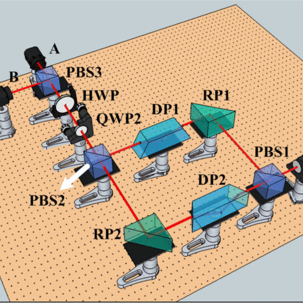
\includegraphics[width=1.00\textwidth]{fig/scheme_clipped.png}
\end{figure}

\column{0.60\textwidth}
\begin{align}
    \ket{H}\otimes\ket{m} &\to \frac{1}{\sqrt{2}}(\exp(i m \theta)\ket{L}\nonumber\\
    &+ \exp(-i m \theta)\ket{R})\otimes\ket{m} \\\nonumber\\
    = (\cos(m & \theta)\ket{H}+\sin(m \theta)\ket{V})\otimes\ket{m}
\end{align}

\hspace{8pt} Via the final HWP one gains access of more possible projecting basis.

\end{columns}
\end{frame}

\section{MZI-like rotation detecting: scheme 1}

\begin{frame}{Rotation detecting based on PRL scheme}

DP2 replaced by cavity, $m\theta\to\pi/4$:
\begin{align}
    \ket{m(t)} :&= \exp(i m\Omega t)\ket{m}, t^\prime = t-1/(\nu_{FSR}T) \\ 
    \ket{H}\otimes\ket{m(t)} &\to \frac{1}{2}((1+i)\ket{L}\otimes\ket{m(t^\prime)} + (1-i)\ket{R}\otimes\ket{m(t)} \nonumber \\ 
    = \ket{\Psi} &= \frac{1}{\sqrt{2}}(\left(1+\frac{1-i}{2}\delta\right)\ket{H}+\left(1-\frac{1+i}{2}\delta\right)\ket{V})\otimes\ket{m(t)}
\end{align}
Projecting measurement @PBS3 gives balance signal:
\begin{align}
    B &= \left|\braket{H|\Psi}\right|^2 - \left|\braket{V|\Psi}\right|^2 = \delta = \frac{m \Omega}{\nu_{FSR}T}
\end{align}
    
\end{frame}

\begin{frame}{Rotation detecting based on PRL scheme: note}
...But this lucid method cannot be directly used in our setup,
\begin{itemize}
    \item State needed:$\ket{m(t)}$
    \item $\delta$ is sign-sensitive.
    \item For $\ket{\psi(t)}=e^{i m\Omega t}\ket{m}+e^{-i m\Omega t}\ket{-m}$, \\
    \hspace{10pt} two components will \textcolor{suoh}{cancel each other.}
\end{itemize}
    
\end{frame}

\section{MZI-like rotation detecting: scheme 2}

\begin{frame}{Rotation detecting: original}

Dove prism angle $m\theta\to\pi/2$
\begin{itemize}
    \item On path 1, $\ket{\psi(t)}$ is rotated to $\ket{\tilde{\psi}(t)}=e^{i m\Omega t}\ket{m}-e^{-i m\Omega t}\ket{-m}$
    \item On path 2, $\ket{\psi(t)}$ is delayed by cavity, $\ket{\psi(t)}\to\ket{\psi(t^\prime)}$ 
    \item $\ket{\tilde{\psi}(t)}$'s polarization is then rotated to $\ket{H}+i\ket{V}$, $\ket{\psi(t^\prime)}$ to $\ket{H}-i\ket{V}$ by QWP.
\end{itemize}


A PZT scanner is introduced to modulate phase difference $\varphi$ of MZI arms.    

\end{frame}

\begin{frame}{Rotation detecting: original}

Calculating amplitude of interference at final PBS:
\begin{subequations}
\begin{align}
    \ket{\psi_1} &= \frac{1}{\sqrt{2}}(\ket H + i\ket V)\otimes\ket{\tilde{\psi}(t)} \\
    \ket{\psi_2} &= \frac{1}{\sqrt{2}}(\ket H - i\ket V)\otimes\ket{\psi(t^\prime)}
\end{align}
\end{subequations}    
\begin{align}
    B &= |\bra{H}(\ket{\psi_1}+\ket{\psi_2})|^2 - |\bra{V}(\ket{\psi_1}+\ket{\psi_2})|^2 \nonumber\\
    &= \left|\frac{e^{i m \Omega t}}{2}\left(1+e^{i\left(\varphi-\frac{m \Omega}{\nu_{FSR}T}\right)}\right)\right|^2 + \left|\frac{e^{-i m \Omega t}}{2}\left(-1+e^{i\left(\varphi+\frac{m \Omega}{\nu_{FSR}T}\right)}\right)\right|^2 -1 \nonumber\\
    &= -\sin\left(\frac{m \Omega}{2 \nu_{FSR}T}\right)\sin \frac{\varphi}{2}
\end{align}
\end{frame}

\begin{frame}{Rotation detecting: original - discussion}

This method may work for our superposition phase plate.
\begin{itemize}
    \item Comparing with PRL scheme, coefficient is halved.
    \item balance detector has to be used in both schemes to form a homodyne detection and subtract two strong background signals. For the second scheme, a lock-in amplifier also has to be employed to extract periodic raw signal. 
    \item for best effect, scan amplitude of PZT should be $\lambda$.
\end{itemize}

    
\end{frame}

\end{document}